\section{Online Advice at a Fixed Request
Budget}\label{online-advice-at-a-fixed-request-budget}

\begin{longtable}[]{@{}
  >{\raggedright\arraybackslash}p{(\linewidth - 10\tabcolsep) * \real{0.1667}}
  >{\raggedright\arraybackslash}p{(\linewidth - 10\tabcolsep) * \real{0.1667}}
  >{\raggedleft\arraybackslash}p{(\linewidth - 10\tabcolsep) * \real{0.1667}}
  >{\raggedleft\arraybackslash}p{(\linewidth - 10\tabcolsep) * \real{0.1667}}
  >{\raggedright\arraybackslash}p{(\linewidth - 10\tabcolsep) * \real{0.1667}}
  >{\raggedleft\arraybackslash}p{(\linewidth - 10\tabcolsep) * \real{0.1667}}@{}}
\caption{Online-advice comparison on ten fresh paired seeds per setting
at initial imitation weight 0.1. Request caps equal the selected bank's
construction-and-checking requests. The online model receives the same
full-map consultation prompt used for rule generation. The comparison
replaces the earlier unequal 15/12-pair study in the main
text.}\tabularnewline
\toprule\noalign{}
\begin{minipage}[b]{\linewidth}\raggedright
Task
\end{minipage} & \begin{minipage}[b]{\linewidth}\raggedright
Student
\end{minipage} & \begin{minipage}[b]{\linewidth}\raggedleft
Request cap
\end{minipage} & \begin{minipage}[b]{\linewidth}\raggedleft
Bank minus online AUC
\end{minipage} & \begin{minipage}[b]{\linewidth}\raggedright
95\% CI
\end{minipage} & \begin{minipage}[b]{\linewidth}\raggedleft
Holm-adjusted \(p\)
\end{minipage} \\
\midrule\noalign{}
\endfirsthead
\toprule\noalign{}
\begin{minipage}[b]{\linewidth}\raggedright
Task
\end{minipage} & \begin{minipage}[b]{\linewidth}\raggedright
Student
\end{minipage} & \begin{minipage}[b]{\linewidth}\raggedleft
Request cap
\end{minipage} & \begin{minipage}[b]{\linewidth}\raggedleft
Bank minus online AUC
\end{minipage} & \begin{minipage}[b]{\linewidth}\raggedright
95\% CI
\end{minipage} & \begin{minipage}[b]{\linewidth}\raggedleft
Holm-adjusted \(p\)
\end{minipage} \\
\midrule\noalign{}
\endhead
\bottomrule\noalign{}
\endlastfoot
DoorKey-8 & PPO & 62 & +.937 & {[}.921, .953{]} &
\(1.5\times10^{-15}\) \\
DoorKey-8 & Count-PPO & 62 & +.360 & {[}.038, .682{]} & .065 \\
MultiRoom-N6 & PPO & 36 & +.738 & {[}.655, .821{]} &
\(2.7\times10^{-8}\) \\
MultiRoom-N6 & Count-PPO & 67 & +.101 & {[}\ensuremath{-}.047, .250{]} & .156 \\
\end{longtable}

Online advice supplies mean label counts of 61.5 and 59.2 for DoorKey
PPO and Count-PPO, and 35.7 and 65.4 for the corresponding MultiRoom
students. Banks supply approximately 1.81M, 1.93M, 3.20M and 0.83M
labels per run, respectively. This is a request-budget comparison, not a
matched-supervision experiment. The reported selected-bank cost excludes
unused development candidates and student training compute.




\begin{figure}[tp]\centering
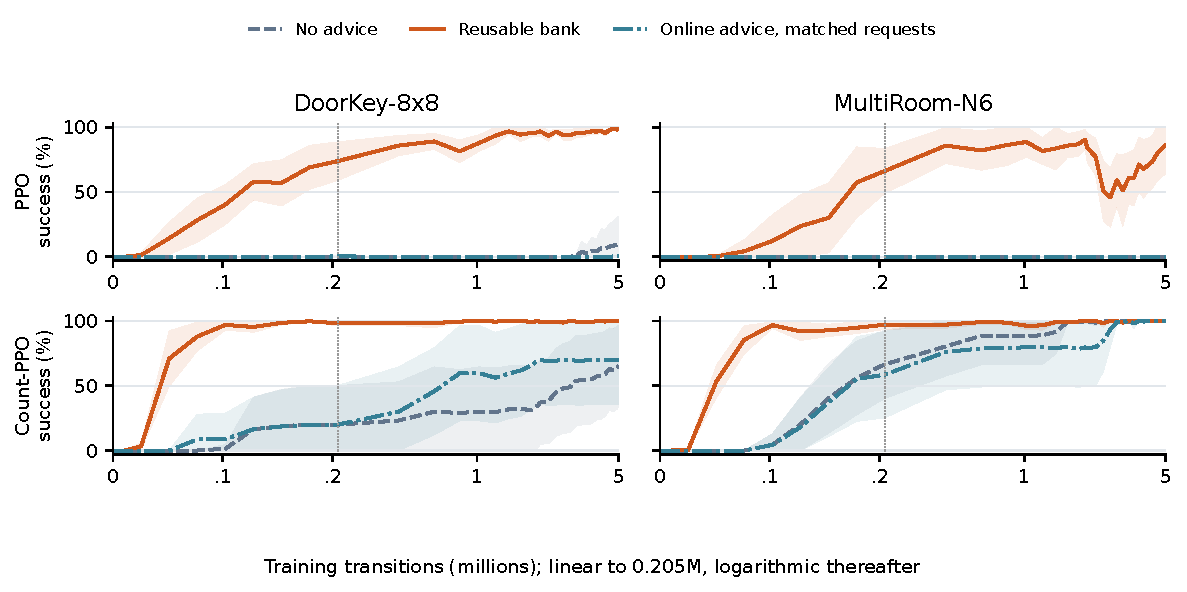
\includegraphics[width=\linewidth]{figures/online_learning.pdf}
\caption{Reusable bank versus online advice with a matched request cap. Ten fresh paired seeds per setting and 5M transitions. Initial and early checkpoints are measured; the axis is linear through 204,800 transitions and logarithmic thereafter. Curves are mean teacher-free greedy success with pointwise unadjusted 95\% $t$-intervals across training seeds, clipped to the feasible range. Curve-band overlap is not a test of paired AUC differences.}
\end{figure}
